% -%-%-%-%-%-%-%-%-%-%-%-%-%-%-%-%-%-%-%-%-%-%-%-%-%
% FLE % 
% Data:28/11/2011                                 %
% Paris,France                                    % 
% Groupe:                                         %
% - Tiago Chedraoui Silva                   % 
% - Angie Anazgo la Rosa %
% -%-%-%-%-%-%-%-%-%-%-%-%-%-%-%-%-%-%-%-%-%-%-%-%-%

\documentclass[a4paper,11pt]{article}

\usepackage[francais,listings,algo]{tcs}

% Cover %
\def \ttprofname{Roland BADEAU} % teachers name
\def \ttabrv{MDI224} % abbreviation of names class
\def \ttabrvxt{} % period
\def \mytitle{Interpolation par splines cubiques} % Big title
\def \mysubtitle{ Travaux Pratique 1 - Deuxième semestre de 2011} % subtitle
\def \ttauthi{} % author's name
\def \ttxti{} % Extra text right side of name
\def \ttauthii{Tiago Chedraoui Silva} % author's name
\def \ttxtii{Casier: 214 } % Extra text right side of name
\def \ttdate{Décembre 15, 2011} % date

\begin{document}
\titleTMB 
\newpage
\tableofcontents
\newpage

\section{Résolution du système linéaire}

\subsection{Méthode de Jacobi}
\subsubsection{Implémentation}

\begin{multicols}{2}
  \lstinputlisting[title=\textbf{Méthode de Jacobi}]{../jacobi.m}
\end{multicols}

\newpage
\subsubsection{Convergence}
\begin{figure}[h!]
  \begin{centering}
    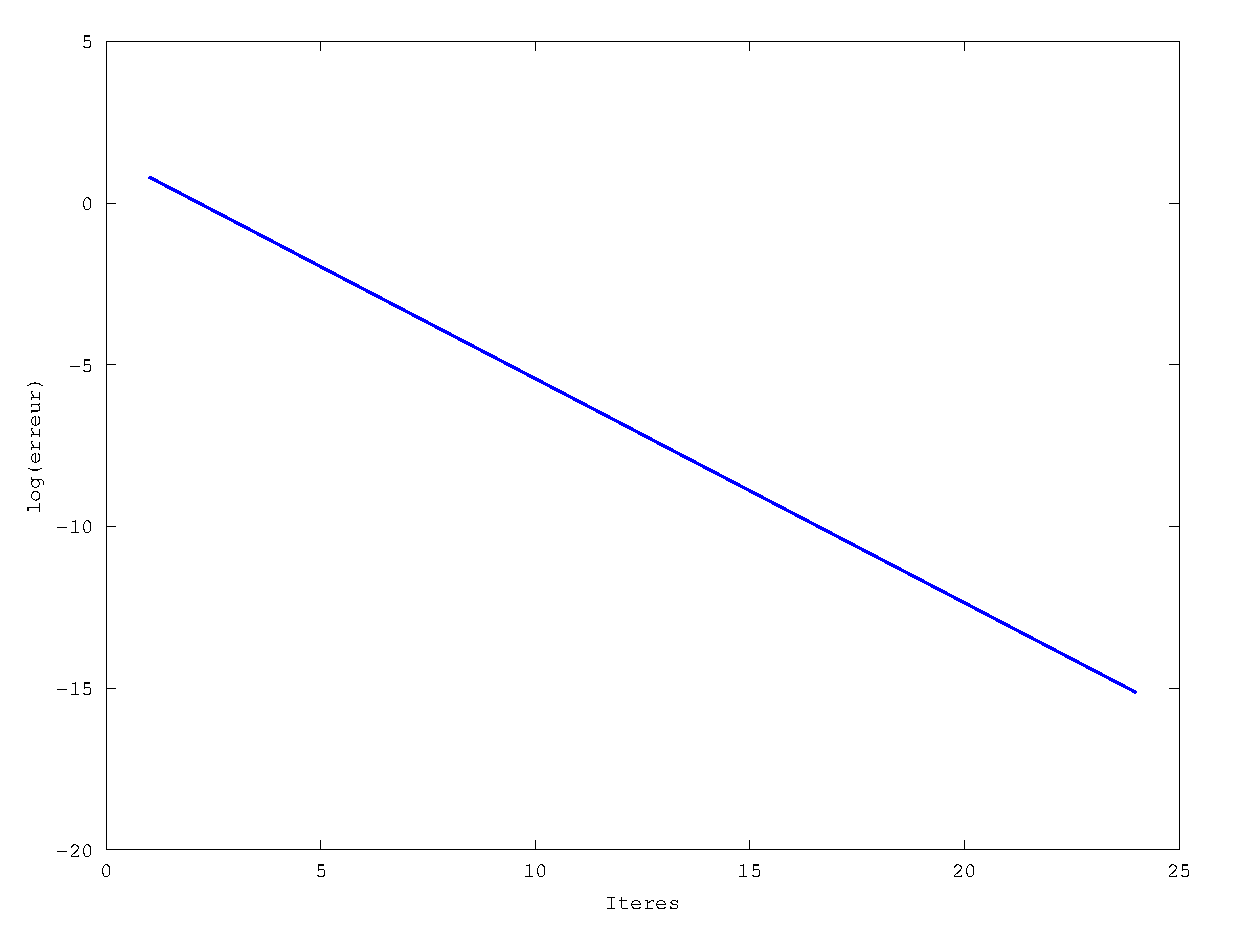
\includegraphics[scale=0.5]{../jacobi_graph}
    \label{rspro2}
    \par\end{centering}
  \caption{Convergence de la méthode de Jacobi}
  \label{fig:jacobi-conv}
\end{figure}

En utilisant la fonction polyfit, nous avons trouvé le polynome: 
$p(x)= -0.693147 x + 1.903331 $


\subsection{Méthode de relaxation}
\subsubsection{Implémentation}
\begin{multicols}{2}
  \lstinputlisting[title=\textbf{Méthode de Jacobi}]{../relax.m}
\end{multicols}

\subsubsection{Convergence}
\begin{figure}[h!]
  \begin{centering}
    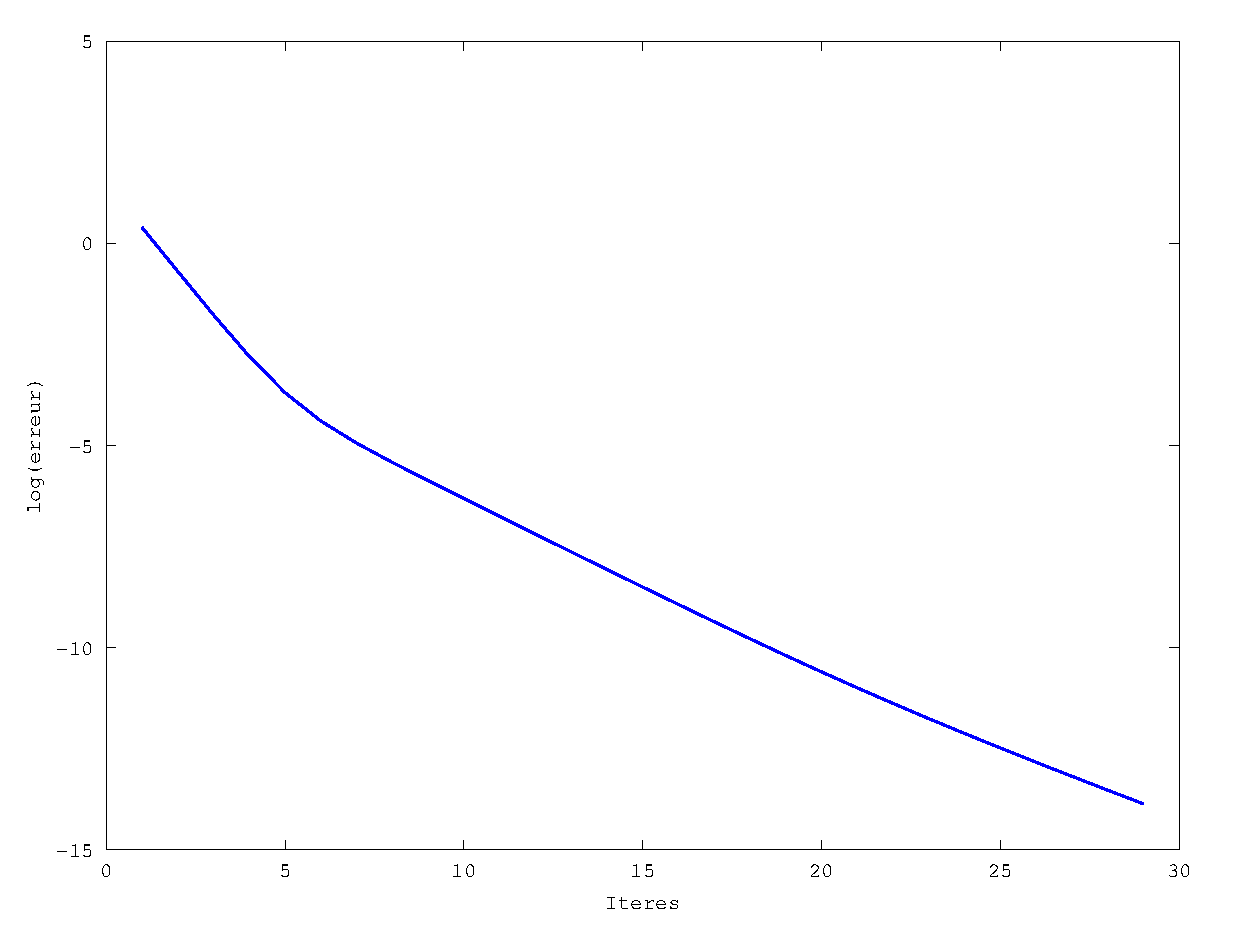
\includegraphics[scale=0.5]{../relaxation_graph}
    \label{rspro2}
    \par\end{centering}
  \caption{Convergence de la méthode de Relaxation pour w=0.5}
  \label{fig:jacobi-conv}
\end{figure}


\begin{figure}[h!]
  \begin{centering}
    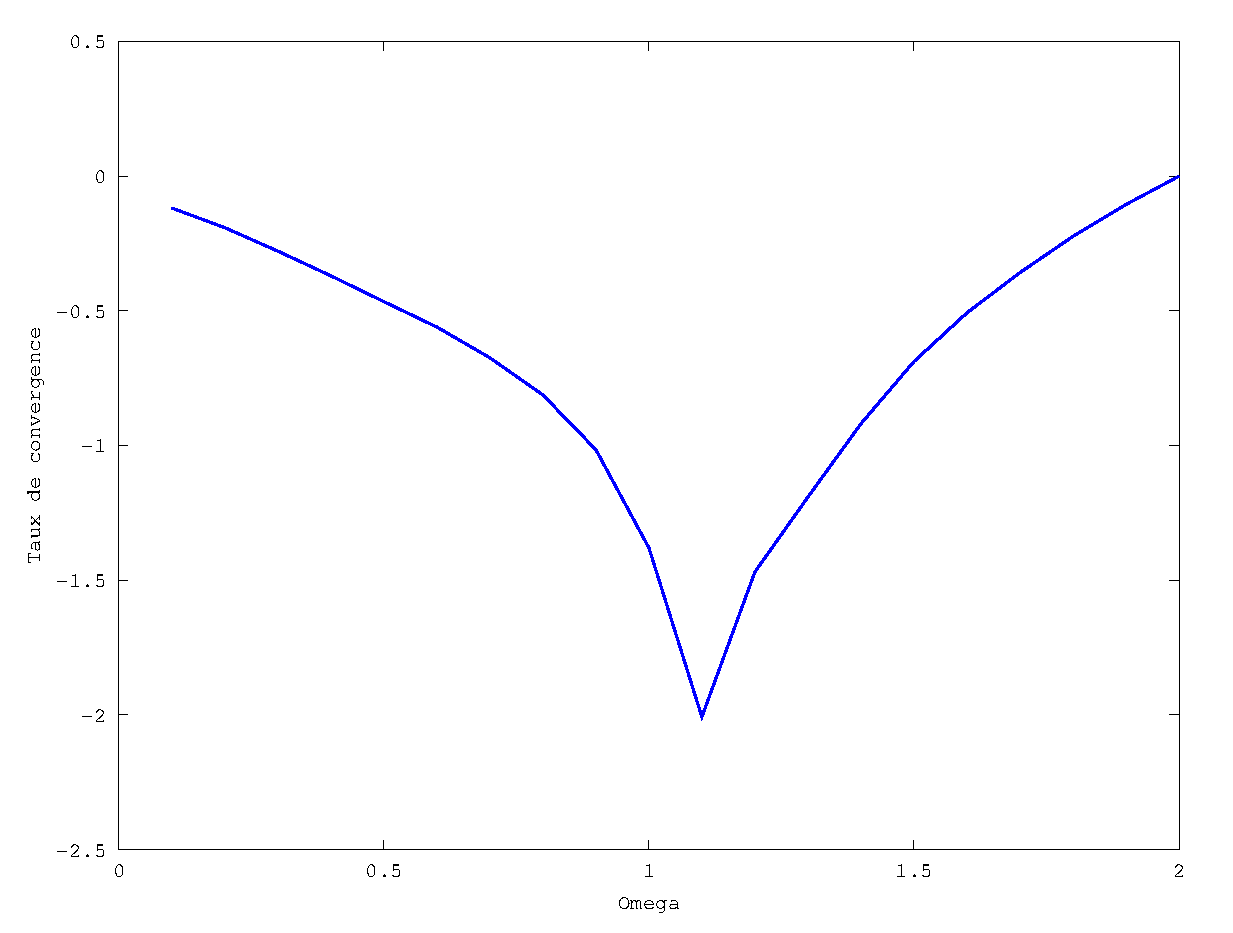
\includegraphics[scale=0.5]{../relaxation_conv}
    \label{rspro2}
    \par\end{centering}
  \caption{Taux de convergence en fonction du paramètre de relaxation w}
  \label{fig:jacobi-conv}
\end{figure}

\subsection{Méthode de Cholesky}
\subsubsection{Implémentation}
\subsubsection{Complexité}

\section{Application}
\subsection{Calcul d'une spline d'interpolation}
\subsection{Évaluation d'une fonction spline cubique}
\subsection{Application}

\end{document}